%!TEX root = paper.tex

\section{Results}
\label{sec:org99c3fc8}
In the following, we evaluate the forecast quality of our method compared to
multiple state-of-the-art forecasts for confirmed cases on
county-level. All comparison forecasts are collected from the COVID-19 Forecast
Hub\footnote{\url{https://github.com/reichlab/covid19-forecast-hub}} as submitted by
the respective teams. The COVID-19 Forecast Hub features weekly county-level forecasts.  
We've chosen the top performing models that have been submitted and chosen dates to 
maximize overlap between models.  The full list of comparison forecasts is shown in \Cref{tab:forecasts}.
\todo{Reconcile models between old evaluation and new evaluation tables}

\begin{table*}[t]
\small
\caption{Forecasting models for confirmed cases on county-level.\label{tab:forecasts}}
\centering
\begin{tabular}{lll}
\toprule
\bf Group & \bf Model \\
\midrule
Center for Disease Dynamics, Economics \& Policy & \it CDDP-SEIR\_MCMC & \citep{cddep_seir_mcmc} \\
Columbia University & \it CU-* & \citep{forecasts/columbia} \\
COVID Alliance at MIT & \it MITCovAlliance-SIR & \citep{baek2020limits} \\
Iowa State University Lily Wang Research Group & \it IowaStateLW-STEM & \citep{wang2020spatiotemporal} \\
Johns Hopkins ID Dynamics COVID-19 Working Group & \it JHU-IDD\_CovidSP & \citep{forecasts/jhu_idd_covidsp} \\
LockNQuay & \it LNQ-ens1 & \citep{forecasts/lnq_ens1} \\
Oliver Wyman & \it Pandemic Navigator & \citep{forecasts/oliver_wyman} \\
UCLA Statistical Machine Learning Lab & \it UCLA-SuEIR & \citep{forecasts/Zou2020.05.24.20111989} \\
University of Southern California Data Science Lab & \it USC-SI\_kJalpha & \citep{srivastava2020fast} \\
University of Massachusetts Amherst & \it UMass-MechBayes & \citep{forecasts/umass_mechbayes} \\
Google and Harvard University & \it Google\_Harvard-CPF & \citep{forecasts/google} \\
Microsoft & \it Microsoft-DeepSTIA & \citep{forecasts/microsoft} \\
University of Virginia & \it UVA-Ensemble & \citep{forecasts/uva} \\
University of Georgia & \it CEID-Walk & \citep{forecasts/ceid} \\
Los Alamos National Labs & \it LANL-GrowthRate & \citep{forecasts/lanl} \\
\bottomrule
\end{tabular}
\end{table*}

\paragraph{Forecast setup and model selection} To compute forecasts for the
different dates, we use the following fully automated model
selection scheme: For each forecast date \(d\), we perform cross-validation by
holding out 7 days of validation data and train the model on the
remaining data. We then select the best hyperparameters as measured by MAE on
the held out validation set and retrain the whole model with those hyperparameters on the
combined training and validation set to compute the final forecast. When
computing the forecasts, we hold all additional input data (e.g., symptom
survey, mobility, weather, etc.) constant after the last observed day
\(d\).\footnote{This setting places natural limits on the duration of the forecasting
horizon. We reserve the joint forecasting of cases and covariates -- what could
extend the horizon -- for future work.}. For all training details of the model,
please see the supplementary material.


\paragraph{Input data} As input features for \bAR, we use multiple data sources
as listed in \Cref{tab:data-sources}. Confirmed cases enter the model only in the
autoregressive part. All other covariates enter the model only as input features
for the time-varying \(\beta\)-part. For cases and weather data, we use the
preprocessed data from the Google COVID-19 Open Data repository
\citep{data/Wahltinez2020}. All datasets are publicly available, de-identified,
and aggregated at county- or state-level.  For data that only exists at the state-level,
we pass the state-level value in for each county in the state.

\begin{table*}[t]
\small
\caption{Data sources for \bAR.\label{tab:data-sources}}
\centering
\begin{tabular}{lll}
\toprule
\bf Dataset & \bf Source & \bf Resolution \\
\midrule
Confirmed Cases &  \citet{data/nytimes_cases} &  County \\
& \multicolumn{1}{l}{\it Confirmed cases based on reports from state \& local health agencies} \\
\midrule
Symptom Survey & CMU COVIDcast \citep{data/covidcast} & County, State \\
& \citet{data/fb_symptom_survey} \\
& \multicolumn{1}{l}{\it Prevalence of COVID-like symptoms from self-reported surveys} \\
\midrule
Movement Range Maps &  \citet{data/fb_movement_range} &  County, State \\
& \multicolumn{1}{l}{\it Mobility metrics related to physical distancing measures} \\
& \multicolumn{1}{l}{\it (change in movement and staying put)} \\
\midrule
Community Mobility & \citet{data/google_mobility} &  County, State \\
& \multicolumn{1}{l}{\it Movement trends across different categories of places} \\
& \multicolumn{1}{l}{\it (retail and recreation, groceries and pharmacies, etc.)} \\
\midrule
Doctor visits & CMU COVIDcast \citep{data/covidcast} & County, State \\
& \multicolumn{1}{l}{Percentage of COVID-related doctor’s visits in a given location} \\
\midrule
Testing &  \citet{data/covidtracking} & State \\
& \multicolumn{1}{l}{\it Total number of COVID PCR tests per state} \\
\midrule
Weather & NOAA GHCN \citep{data/menne2012overview} &  County \\
& \multicolumn{1}{l}{\it Average, minimum, maximum temperature \& rainfall per county} \\
\bottomrule
\end{tabular}
\end{table*}

\begin{figure}[t]
  \centering
  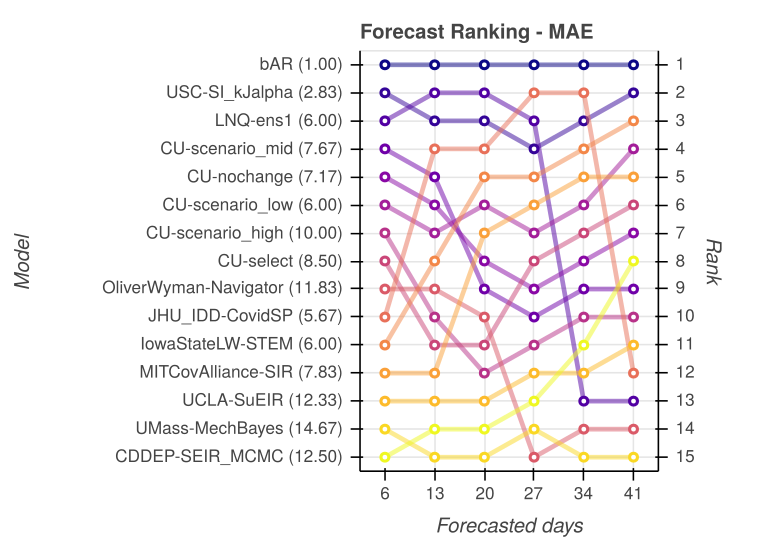
\includegraphics[width=\columnwidth]{img/us_rank_mae.png}
  \vspace{-2ex}
\caption{Ranking of county-level forecasts by average MAE over various forecast horizons. The proposed neural relational autoregressive model (\bAR) shows strong performance over all horizons when compared to state-of-the-art forecasts. Mean rank over all horizons in parentheses.}
\label{fig:ranking-covidhub-mae}
\end{figure}


\paragraph{Forecast evaluation} \Cref{tab:reichalb_eval_1} - \Cref{tab:reichalb_eval_4} show the forecast quality as measured by MAE for multiple forecast horizons.  
The COVID-19 Forecast Hub requires submissions to be in weekly format, where each forecast predicts the number of new cases each week (see \citep{reichlab} for more details about submission format).  
The proposed \bAR model shows consistently strong performance, especially for further out time horizons (2-4 weeks).  


%\paragraph{Forecast evaluation} \Cref{fig:mae-covidhub} shows the forecast
%quality as measured by MAE for multiple forecast horizons.\footnote{MAE numbers are computed in accordance with \url{https://github.com/youyanggu/covid19-forecast-hub-evaluation}} It can be seen that
%the proposed \bAR models shows a consistently strong performance and is for all
%forecasting dates and horizons either the best model or among the best.
%\Cref{fig:ranking-covidhub-mae}, which shows the ranking of all models by the
%average MAE for each forecast horizon, further illustrates this property. It can
%be seen that \bAR model is consistently ranked first over all horizons.
%Furthermore, other models show much larger variability in their performance.

\begin{figure*}[t]
\centering
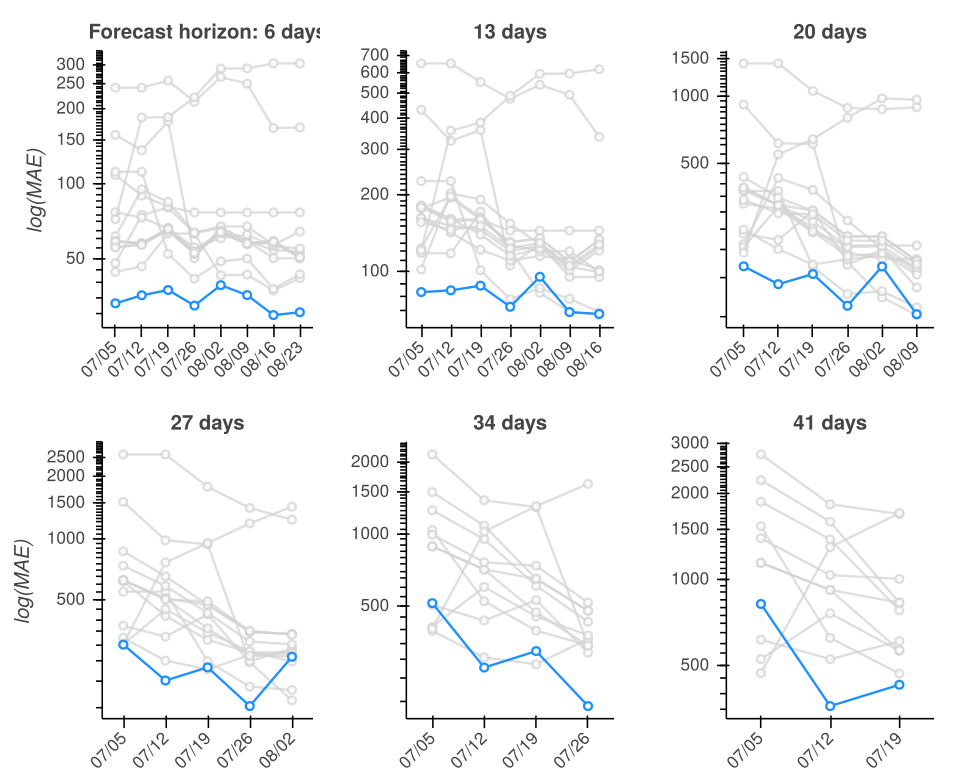
\includegraphics[width=.75\linewidth]{img/us_mae/us_mae.png}
\caption{\label{fig:mae-covidhub}Comparison of \bAR model (blue) to 15 county-level models from COVID-19 forecast hub (gray). Forecast quality is measured in MAE (log-scale) where the absolute errors are averaged over all counties. For similar analysis using RMSE please see the supplementary material.}
\end{figure*}


To also evaluate the performance of our model on days prior to July 5th, we
compare to forecasts of Google Cloud AI \citep{arik2020interpretable} and Columbia
University \citep{forecasts/columbia} which provide county-level forecasts of
confirmed cases from May 11th to June 27th. \Cref{fig:mae-google} shows the average
MAE over all counties for 7 and 14 day forecasts for these models.\footnote{For this
comparison, average MAE is computed as described in \citep{arik2020interpretable}}
It can be seen that the \bAR model shows again consistently strong performance on these
earlier days and is typically ranked first for both 7 and 14 day forecasts.

\begin{figure*}[t]
\centering
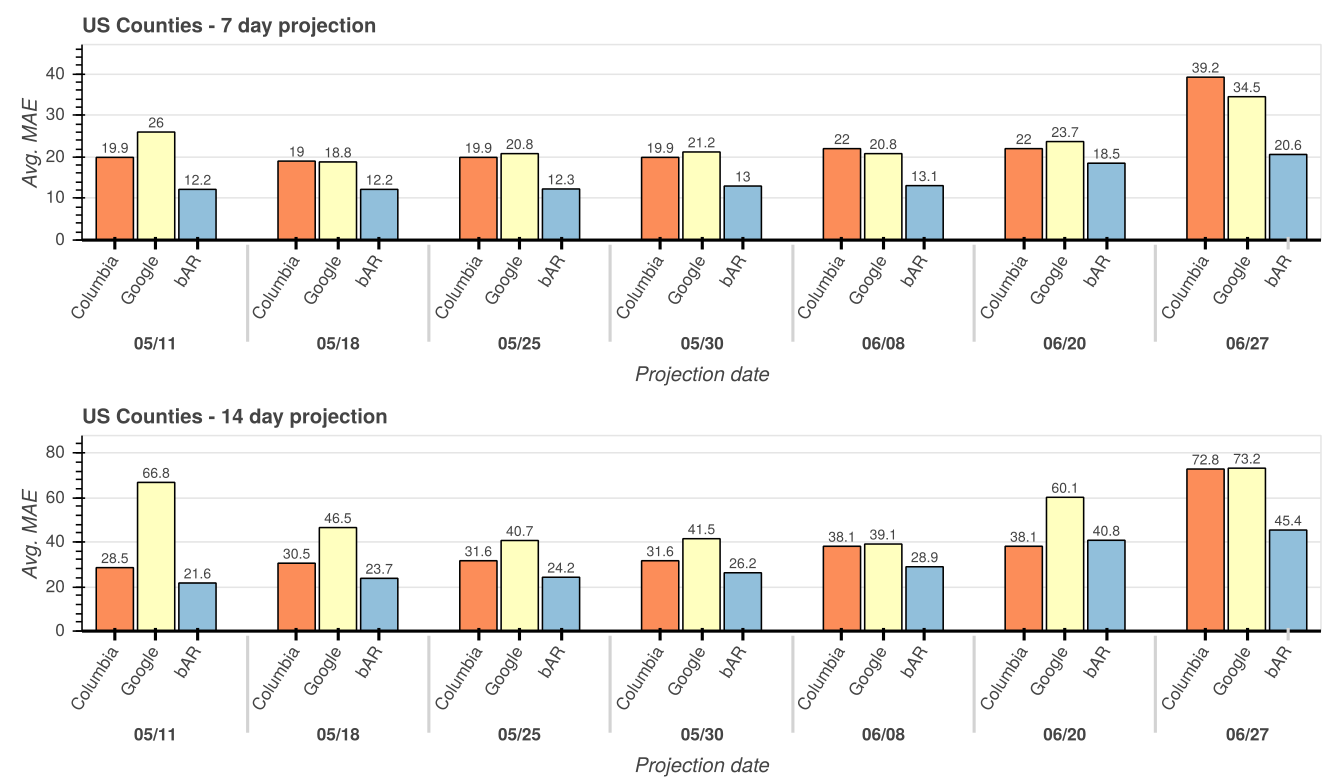
\includegraphics[width=.9\textwidth]{img/counties_bar_mae.png}
\caption{\label{fig:mae-google}Comparions of \bAR model to forecasts from Google Cloud AI and Columbia for 7 and 14 day horizons and earlier forecast dates. Forecast quality is measured in MAE where the absolute errors are averaged over all counties.}
\end{figure*}

\begin{figure*}[t]
\centering
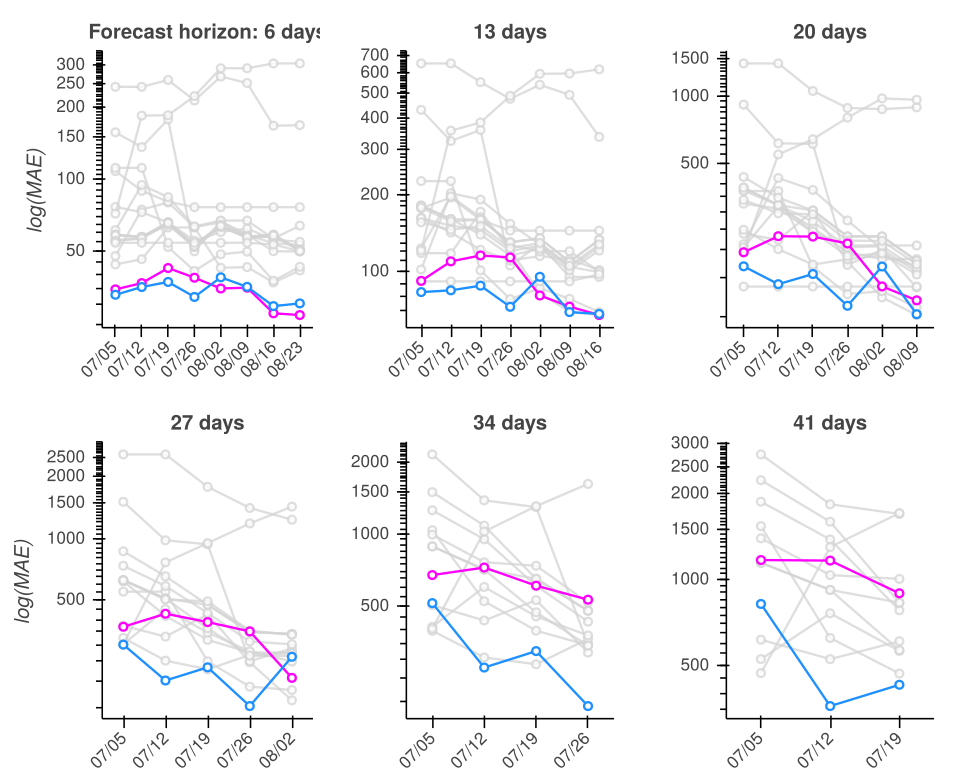
\includegraphics[width=.9\columnwidth]{img/us_mae_granger_ablation/us_mae_granger_ablation.png}
\hfil
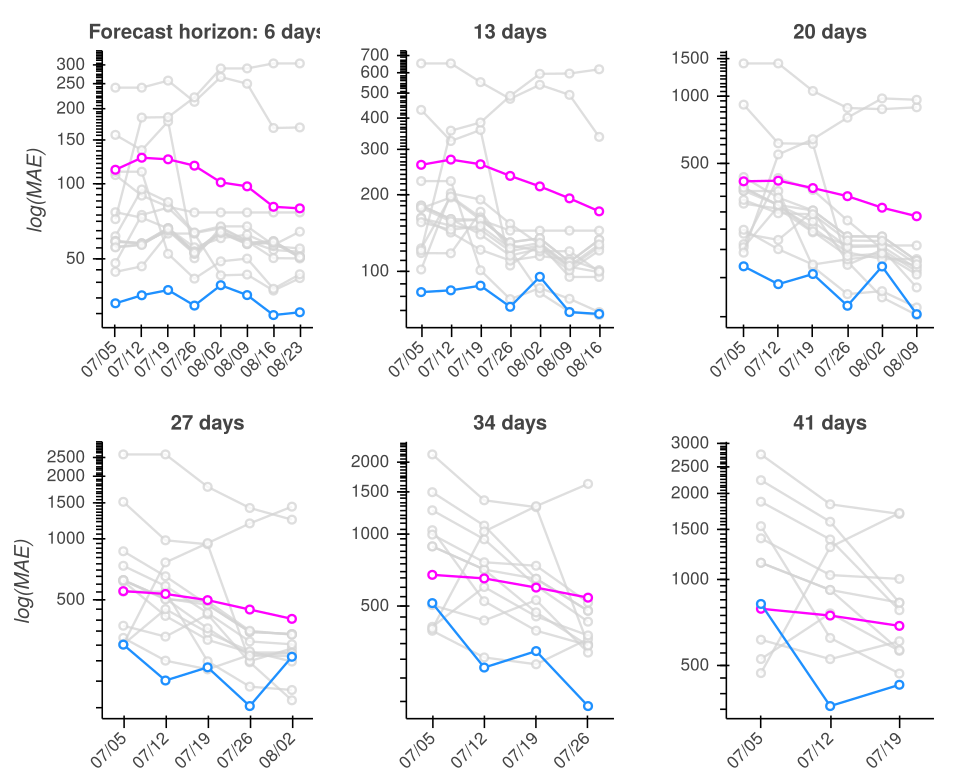
\includegraphics[width=.9\columnwidth]{img/us_mae_loss_ablation/us_mae_granger_ablation.png}
\caption{\label{fig:mae-covidhub-granger}Comparison of \bAR model with (blue) and without (magenta) Granger regularization. Forecast quality is measured in MAE.}
\end{figure*}


\paragraph{Ablations} In addition to comparisons to state-of-the-art
county-level forecasts, we also evaluate the contributions of different aspects
of our model. First, we test the effect of the relational autoregressive part.
For this purpose, we trained additional models were we disabled the relational
part (by setting \(\forall i \neq j: w_{ij} = 0\)) and compared their forecasts to
the full model of \Cref{eq:beta-ar}. To measure the relative improvement of the
full model over the non-relational model, we compute then the relative error of
both models, e.g.,
\begin{equation*}
    \text{Relative Mean Absolute Error} = \frac{\text{MAE}_{\text{full}}}{\text{MAE}_\text{non-relational}}
\end{equation*}
It can be seen from \Cref{fig:quality-ratio} that full model offers substantial
improvements over the non-relational model as the relative forecast quality
grows exponentially with the forecasting horizon. While the non-relational model
can offer acceptable forecast for horizons of 1-2 days, it quickly deteriorates
with larger horizons. This show the importance of the relational component for
disentangling the different growth factors and learning high quality models.

\begin{figure}[tb]
\centering
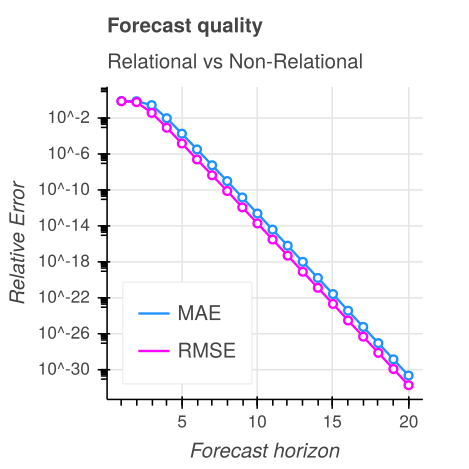
\includegraphics[width=.7\linewidth]{img/quality_ratio.png}
\caption{\label{fig:quality-ratio}Relative Error (MAE and RMSE) of the fully relational \bAR model compared to a non-relational variant.}
\end{figure}


In addition to the non-relational component, we also evaluated the contributions
of the logit-normal regularization method. For this purpose, we trained a model
where we explicitly set the reqularization parameter \(\sigma = 0\). We then
compare the forecast quality to the standard model where the regularization
parameter has been selected via cross-validation. \Cref{fig:mae-covidhub-granger}
shows the results of the comparison. It can be seen that the logit-normal
regularization can be very beneficial to improve forecast quality. While the
differences to the standard model are much smaller than for the non-relational
model, the addition of the regularization term can lead to substantial
improvements, especially for horizons of 13 days and longer.

Finally, we also evaluated the contributions of the Negative Binomial
distribution compared to a standard Poisson distribution for modeling confirmed
cases. Similar to the logit-normalization method, we trained an additional model
with Poisson likelihood and compared the forecast quality to the standard model.
It can be seen from \Cref{fig:mae-covidhub-loss}, that Negative Binomial likelihood
significantly improves the quality of the model over all forecast horizons. This
is likely due to the fact that the Negative Binomial can better model the noise
in the observed data, while the stricter Poisson likelihood causes the
(recurrent) model to overfit to these variations.

\begin{figure}[t]
\centering
\caption{\label{fig:mae-covidhub-loss}Comparison of \bAR model with Negative Binomial (blue) and Poisson (magenta) likelihood. Forecast quality is measured in MAE.}
\end{figure}


\begin{figure}
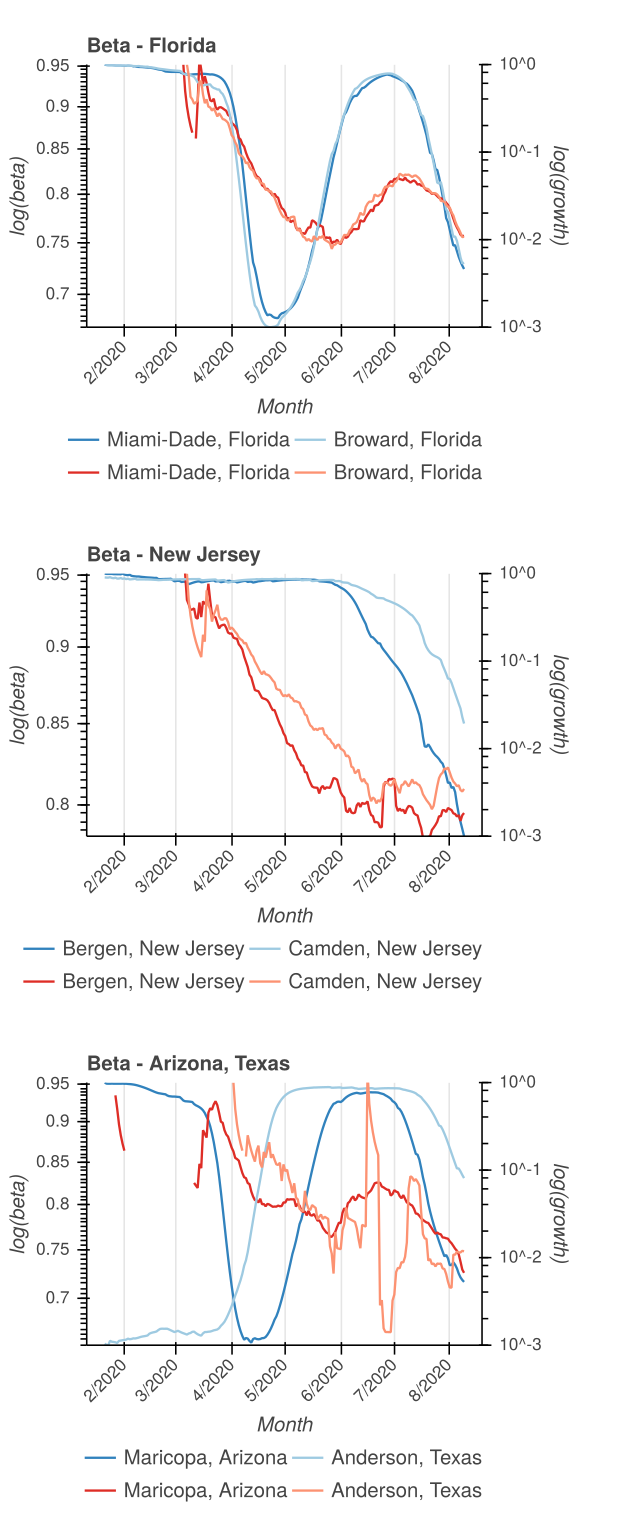
\includegraphics[width=\columnwidth]{img/betas.png}
\caption{Evolution of \(\beta\) over time}
\end{figure}


\begin{table*}[t]
\small
\caption{COVID-19 Forecast Hub MAE (1 week horizon).\label{tab:reichalb_eval_1} }

\centering
    
\begin{tabular}{ccccccccc}
\toprule
{} &                           CEID &       CU &                         $\bAR$ & Google\_Harvard &                           LANL &                            LNQ &                     Microsoft &      UVA \\
basedate   &                                &          &                                &                 &                                &                                &                               &          \\
\midrule
2020-08-06 &                              - &   70.681 &   {\cellcolor{blue!25} 58.610} &               - &                         90.897 &                              - &                             - &        - \\
2020-08-13 &                              - &   61.309 &   {\cellcolor{blue!25} 53.553} &               - &                         74.575 &                              - &                             - &        - \\
2020-09-03 &                              - &   51.492 &   {\cellcolor{blue!25} 43.194} &               - &                         67.363 &                              - &                             - &        - \\
2020-09-27 &                         32.736 &   43.166 &                         36.189 &          42.139 &                              - &   {\cellcolor{blue!25} 23.982} &                             - &        - \\
2020-10-01 &                              - &        - &   {\cellcolor{blue!25} 59.339} &               - &                        101.979 &                              - &                             - &        - \\
2020-10-11 &                          32.27 &   37.986 &                         45.747 &          76.775 &                              - &   {\cellcolor{blue!25} 26.884} &                             - &        - \\
2020-10-15 &                              - &   91.446 &   {\cellcolor{blue!25} 80.918} &               - &                        141.719 &                              - &                             - &        - \\
2020-10-25 &                         48.712 &   52.614 &                         64.412 &          52.371 &                              - &   {\cellcolor{blue!25} 42.044} &                             - &        - \\
2020-11-08 &                              - &   90.748 &                        125.892 &         121.305 &                              - &   {\cellcolor{blue!25} 71.883} &                             - &        - \\
2020-11-15 &                              - &   98.254 &                        113.979 &         118.928 &                              - &   {\cellcolor{blue!25} 73.249} &                             - &        - \\
2020-11-19 &                              - &  181.705 &  {\cellcolor{blue!25} 133.064} &               - &                        180.716 &                              - &                             - &        - \\
2020-12-06 &                              - &  123.796 &                        152.413 &         117.942 &                              - &   {\cellcolor{blue!25} 82.929} &                             - &        - \\
2020-12-07 &  {\cellcolor{blue!25} 102.074} &        - &                        134.868 &               - &                        105.553 &                              - &                             - &  206.377 \\
2020-12-13 &                              - &  105.273 &                        130.788 &         136.166 &                              - &   {\cellcolor{blue!25} 77.028} &                             - &        - \\
2020-12-14 &                        112.741 &        - &                        126.242 &               - &  {\cellcolor{blue!25} 109.234} &                              - &                       116.788 &  347.012 \\
2020-12-17 &                              - &  184.772 &                        179.296 &               - &  {\cellcolor{blue!25} 168.666} &                              - &                             - &        - \\
2020-12-21 &                        125.938 &        - &   {\cellcolor{blue!25} 76.497} &               - &                        138.659 &                              - &                       123.644 &  336.419 \\
2021-01-03 &                              - &  136.050 &                        174.788 &         259.101 &                              - &  {\cellcolor{blue!25} 123.627} &                             - &        - \\
2021-01-04 &                         77.432 &        - &                        156.656 &               - &                        108.324 &                              - &  {\cellcolor{blue!25} 74.025} &  401.928 \\
2021-01-11 &                        129.006 &        - &   {\cellcolor{blue!25} 85.915} &         190.840 &                        110.568 &                              - &                       159.404 &  390.672 \\
2021-01-18 &                        168.776 &        - &   {\cellcolor{blue!25} 74.570} &         207.132 &                        111.241 &                              - &                       134.228 &  424.307 \\
2021-01-25 &                        112.402 &        - &   {\cellcolor{blue!25} 66.138} &          92.175 &                         66.162 &                              - &                        79.503 &  314.897 \\
\bottomrule
\end{tabular}

\end{table*}

    
\begin{table*}[t]
\small
\caption{COVID-19 Forecast Hub MAE (2 week horizon).\label{tab:reichalb_eval_2} }

\centering
    
\begin{tabular}{ccccccccc}
\toprule
{} &     CEID &                             CU &                         $\bAR$ &                Google\_Harvard &     LANL &      LNQ &                      Microsoft &      UVA \\
basedate   &          &                                &                                &                                &          &          &                                &          \\
\midrule
2020-08-06 &        - &                        163.989 &  {\cellcolor{blue!25} 125.481} &                              - &  196.062 &        - &                              - &        - \\
2020-08-13 &        - &                        144.941 &  {\cellcolor{blue!25} 114.155} &                              - &  172.747 &        - &                              - &        - \\
2020-09-03 &        - &                        127.597 &  {\cellcolor{blue!25} 123.920} &                              - &  165.917 &        - &                              - &        - \\
2020-09-27 &   116.03 &                        127.281 &   {\cellcolor{blue!25} 96.989} &                        135.297 &        - &  119.996 &                              - &        - \\
2020-10-01 &        - &                              - &  {\cellcolor{blue!25} 174.502} &                              - &  236.432 &        - &                              - &        - \\
2020-10-11 &  169.718 &                        157.076 &  {\cellcolor{blue!25} 141.673} &                        200.563 &        - &  166.886 &                              - &        - \\
2020-10-15 &        - &                        248.751 &  {\cellcolor{blue!25} 221.959} &                              - &  336.129 &        - &                              - &        - \\
2020-10-25 &  287.529 &                        267.457 &  {\cellcolor{blue!25} 228.184} &                        309.802 &        - &  273.600 &                              - &        - \\
2020-11-08 &        - &                        401.312 &  {\cellcolor{blue!25} 374.674} &                        511.953 &        - &  404.481 &                              - &        - \\
2020-11-15 &        - &                        355.734 &  {\cellcolor{blue!25} 302.691} &                        444.156 &        - &  343.992 &                              - &        - \\
2020-11-19 &        - &                        558.966 &  {\cellcolor{blue!25} 391.979} &                              - &  490.497 &        - &                              - &        - \\
2020-12-06 &        - &                        488.648 &  {\cellcolor{blue!25} 441.784} &                        549.195 &        - &  503.136 &                              - &        - \\
2020-12-07 &  479.261 &                              - &  {\cellcolor{blue!25} 379.099} &                              - &  447.404 &        - &                              - &  461.150 \\
2020-12-13 &        - &                        414.710 &  {\cellcolor{blue!25} 321.997} &                        386.938 &        - &  407.376 &                              - &        - \\
2020-12-14 &  381.172 &                              - &                        313.182 &                              - &  341.375 &        - &  {\cellcolor{blue!25} 311.987} &  399.721 \\
2020-12-17 &        - &                        619.721 &  {\cellcolor{blue!25} 500.558} &                              - &  557.816 &        - &                              - &        - \\
2020-12-21 &  344.883 &                              - &  {\cellcolor{blue!25} 251.703} &                              - &  344.751 &        - &                        301.977 &  325.162 \\
2021-01-03 &        - &  {\cellcolor{blue!25} 473.132} &                        537.502 &                        530.039 &        - &  620.123 &                              - &        - \\
2021-01-04 &  514.208 &                              - &  {\cellcolor{blue!25} 449.326} &                              - &  559.572 &        - &                        576.666 &  477.873 \\
2021-01-11 &  288.342 &                              - &                        227.165 &  {\cellcolor{blue!25} 201.820} &  325.607 &        - &                        276.098 &  364.417 \\
2021-01-18 &  188.991 &                              - &                        147.844 &                        149.761 &  259.540 &        - &  {\cellcolor{blue!25} 134.744} &  295.947 \\
\bottomrule
\end{tabular}

\end{table*}

    
\begin{table*}[t]
\small
\caption{COVID-19 Forecast Hub MAE (3 week horizon).\label{tab:reichalb_eval_3} }

\centering
    
\begin{tabular}{ccccccccc}
\toprule
{} &     CEID &                             CU &                          $\bAR$ &                Google\_Harvard &      LANL &       LNQ & Microsoft &                            UVA \\
basedate   &          &                                &                                 &                                &           &           &           &                                \\
\midrule
2020-08-06 &        - &                        254.378 &   {\cellcolor{blue!25} 202.747} &                              - &   296.812 &         - &         - &                              - \\
2020-08-13 &        - &                        226.903 &   {\cellcolor{blue!25} 194.915} &                              - &   274.213 &         - &         - &                              - \\
2020-09-03 &        - &  {\cellcolor{blue!25} 211.574} &                         223.471 &                              - &   274.117 &         - &         - &                              - \\
2020-09-27 &  233.953 &                        245.834 &   {\cellcolor{blue!25} 200.585} &                        258.717 &         - &   242.927 &         - &                              - \\
2020-10-01 &        - &                              - &   {\cellcolor{blue!25} 320.958} &                              - &   400.305 &         - &         - &                              - \\
2020-10-11 &  345.017 &                        320.967 &   {\cellcolor{blue!25} 294.185} &                        353.256 &         - &   341.595 &         - &                              - \\
2020-10-15 &        - &                        498.298 &   {\cellcolor{blue!25} 435.184} &                              - &   611.468 &         - &         - &                              - \\
2020-10-25 &  608.159 &                        576.229 &   {\cellcolor{blue!25} 492.587} &                        637.124 &         - &   587.218 &         - &                              - \\
2020-11-08 &        - &                        701.287 &   {\cellcolor{blue!25} 660.135} &                        868.373 &         - &   740.942 &         - &                              - \\
2020-11-15 &        - &                        757.398 &   {\cellcolor{blue!25} 615.995} &                        838.653 &         - &   739.112 &         - &                              - \\
2020-11-19 &        - &                       1008.571 &   {\cellcolor{blue!25} 723.106} &                              - &   962.261 &         - &         - &                              - \\
2020-12-06 &        - &                        875.903 &   {\cellcolor{blue!25} 783.316} &                        970.478 &         - &   897.286 &         - &                              - \\
2020-12-07 &  893.938 &                              - &   {\cellcolor{blue!25} 712.124} &                              - &   844.418 &         - &         - &                        814.171 \\
2020-12-13 &        - &                        862.825 &   {\cellcolor{blue!25} 661.099} &                        823.145 &         - &   852.250 &         - &                              - \\
2020-12-14 &  828.416 &                              - &   {\cellcolor{blue!25} 706.945} &                              - &   757.576 &         - &   872.500 &                        712.610 \\
2020-12-17 &        - &                       1165.762 &  {\cellcolor{blue!25} 1026.700} &                              - &  1096.356 &         - &         - &                              - \\
2020-12-21 &        - &                              - &                         765.264 &                              - &   839.919 &         - &   776.512 &  {\cellcolor{blue!25} 734.443} \\
2021-01-03 &        - &  {\cellcolor{blue!25} 790.559} &                         924.455 &                        911.204 &         - &  1023.386 &         - &                              - \\
2021-01-04 &  903.441 &                              - &   {\cellcolor{blue!25} 836.486} &                              - &   934.932 &         - &   933.769 &                        847.050 \\
2021-01-11 &   614.74 &                              - &                         538.522 &  {\cellcolor{blue!25} 436.358} &   630.162 &         - &   723.034 &                        603.746 \\
\bottomrule
\end{tabular}

\end{table*}

    
\begin{table*}[t]
\small
\caption{COVID-19 Forecast Hub MAE (4 week horizon).\label{tab:reichalb_eval_4} }

\centering
    
\begin{tabular}{ccccccccc}
\toprule
{} &     CEID &                              CU &                          $\bAR$ & Google\_Harvard &      LANL &       LNQ & Microsoft &                             UVA \\
basedate   &          &                                 &                                 &                 &           &           &           &                                 \\
\midrule
2020-08-06 &        - &                         343.761 &   {\cellcolor{blue!25} 279.968} &               - &   397.426 &         - &         - &                               - \\
2020-08-13 &        - &                         295.250 &   {\cellcolor{blue!25} 261.564} &               - &   359.325 &         - &         - &                               - \\
2020-09-03 &        - &   {\cellcolor{blue!25} 292.415} &                         320.063 &               - &   377.327 &         - &         - &                               - \\
2020-09-27 &  380.707 &                             385 &   {\cellcolor{blue!25} 336.712} &         410.264 &         - &   394.817 &         - &                               - \\
2020-10-01 &        - &                               - &   {\cellcolor{blue!25} 493.807} &               - &   589.957 &         - &         - &                               - \\
2020-10-11 &  598.004 &                         572.784 &   {\cellcolor{blue!25} 523.691} &         586.931 &         - &   592.813 &         - &                               - \\
2020-10-15 &        - &                         823.338 &   {\cellcolor{blue!25} 712.588} &               - &   956.171 &         - &         - &                               - \\
2020-10-25 &  984.938 &                         955.633 &   {\cellcolor{blue!25} 805.278} &        1010.447 &         - &   961.117 &         - &                               - \\
2020-11-08 &        - &                        1088.816 &   {\cellcolor{blue!25} 996.985} &        1285.209 &         - &  1159.153 &         - &                               - \\
2020-11-15 &        - &                        1255.347 &   {\cellcolor{blue!25} 970.215} &        1279.068 &         - &  1190.497 &         - &                               - \\
2020-11-19 &        - &                        1486.725 &  {\cellcolor{blue!25} 1036.903} &               - &  1487.456 &         - &         - &                               - \\
2020-12-06 &        - &                        1338.241 &  {\cellcolor{blue!25} 1152.662} &        1429.709 &         - &  1336.666 &         - &                               - \\
2020-12-07 &  1346.16 &                               - &  {\cellcolor{blue!25} 1073.909} &               - &  1318.017 &         - &         - &                        1248.655 \\
2020-12-13 &        - &                        1425.998 &  {\cellcolor{blue!25} 1088.174} &        1369.633 &         - &  1377.635 &         - &                               - \\
2020-12-14 &        - &                               - &                        1222.210 &               - &  1309.565 &         - &  1205.770 &  {\cellcolor{blue!25} 1177.781} \\
2020-12-17 &        - &                        1701.340 &  {\cellcolor{blue!25} 1538.276} &               - &  1617.285 &         - &         - &                               - \\
2020-12-21 &        - &                               - &                        1271.774 &               - &  1351.437 &         - &  1422.710 &  {\cellcolor{blue!25} 1158.224} \\
2021-01-03 &        - &  {\cellcolor{blue!25} 1052.719} &                        1255.068 &        1243.796 &         - &  1351.363 &         - &                               - \\
2021-01-04 &   1233.9 &                               - &                        1168.079 &               - &  1257.376 &         - &  1209.617 &  {\cellcolor{blue!25} 1150.167} \\
\bottomrule
\end{tabular}

\end{table*}

